% Options for packages loaded elsewhere
\PassOptionsToPackage{unicode}{hyperref}
\PassOptionsToPackage{hyphens}{url}
%
\documentclass[
  12pt,
]{article}
\usepackage{amsmath,amssymb}
\usepackage{iftex}
\ifPDFTeX
  \usepackage[T1]{fontenc}
  \usepackage[utf8]{inputenc}
  \usepackage{textcomp} % provide euro and other symbols
\else % if luatex or xetex
  \usepackage{unicode-math} % this also loads fontspec
  \defaultfontfeatures{Scale=MatchLowercase}
  \defaultfontfeatures[\rmfamily]{Ligatures=TeX,Scale=1}
\fi
\usepackage{lmodern}
\ifPDFTeX\else
  % xetex/luatex font selection
\fi
% Use upquote if available, for straight quotes in verbatim environments
\IfFileExists{upquote.sty}{\usepackage{upquote}}{}
\IfFileExists{microtype.sty}{% use microtype if available
  \usepackage[]{microtype}
  \UseMicrotypeSet[protrusion]{basicmath} % disable protrusion for tt fonts
}{}
\makeatletter
\@ifundefined{KOMAClassName}{% if non-KOMA class
  \IfFileExists{parskip.sty}{%
    \usepackage{parskip}
  }{% else
    \setlength{\parindent}{0pt}
    \setlength{\parskip}{6pt plus 2pt minus 1pt}}
}{% if KOMA class
  \KOMAoptions{parskip=half}}
\makeatother
\usepackage{xcolor}
\usepackage[margin=1in]{geometry}
\usepackage{longtable,booktabs,array}
\usepackage{calc} % for calculating minipage widths
% Correct order of tables after \paragraph or \subparagraph
\usepackage{etoolbox}
\makeatletter
\patchcmd\longtable{\par}{\if@noskipsec\mbox{}\fi\par}{}{}
\makeatother
% Allow footnotes in longtable head/foot
\IfFileExists{footnotehyper.sty}{\usepackage{footnotehyper}}{\usepackage{footnote}}
\makesavenoteenv{longtable}
\usepackage{graphicx}
\makeatletter
\def\maxwidth{\ifdim\Gin@nat@width>\linewidth\linewidth\else\Gin@nat@width\fi}
\def\maxheight{\ifdim\Gin@nat@height>\textheight\textheight\else\Gin@nat@height\fi}
\makeatother
% Scale images if necessary, so that they will not overflow the page
% margins by default, and it is still possible to overwrite the defaults
% using explicit options in \includegraphics[width, height, ...]{}
\setkeys{Gin}{width=\maxwidth,height=\maxheight,keepaspectratio}
% Set default figure placement to htbp
\makeatletter
\def\fps@figure{htbp}
\makeatother
\setlength{\emergencystretch}{3em} % prevent overfull lines
\providecommand{\tightlist}{%
  \setlength{\itemsep}{0pt}\setlength{\parskip}{0pt}}
\setcounter{secnumdepth}{-\maxdimen} % remove section numbering
\ifLuaTeX
  \usepackage{selnolig}  % disable illegal ligatures
\fi
\usepackage{bookmark}
\IfFileExists{xurl.sty}{\usepackage{xurl}}{} % add URL line breaks if available
\urlstyle{same}
\hypersetup{
  hidelinks,
  pdfcreator={LaTeX via pandoc}}

\author{}
\date{\vspace{-2.5em}}

\begin{document}

\begin{titlepage}
\begin{center}
\vspace*{3cm}

\includegraphics[width=10cm]{UCL.png} \\[5cm]

\textbf{\LARGE LACTU 2210 - Project 1} \\[2cm]
\textit{\LARGE Group : A}\\


\vfill
\large
MAJDOUBI HIBA  5818-19-00 \\
RWAWI YOUSRA 7831-24-00 \\[1cm]
\textit{Université catholique de Louvain} \\[2cm]
March 2025


\end{center}
\end{titlepage}

\newpage

\newpage

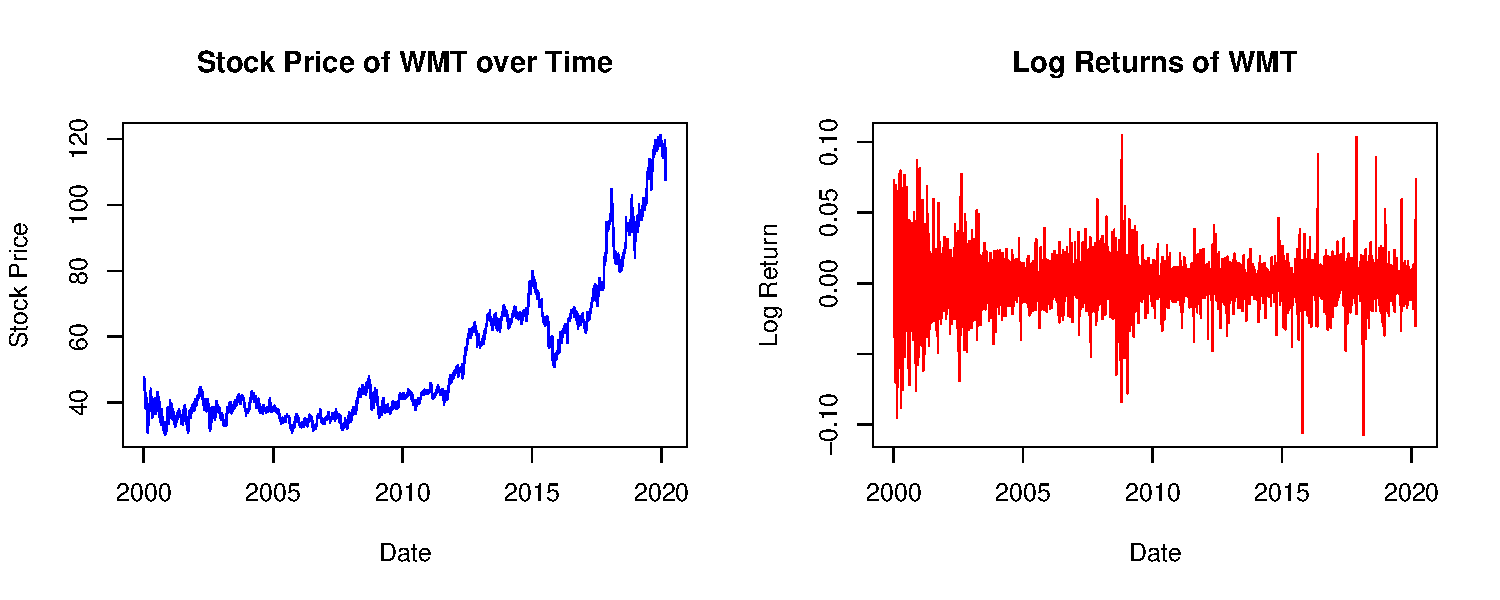
\includegraphics{QRM_files/figure-latex/unnamed-chunk-3-1.pdf}
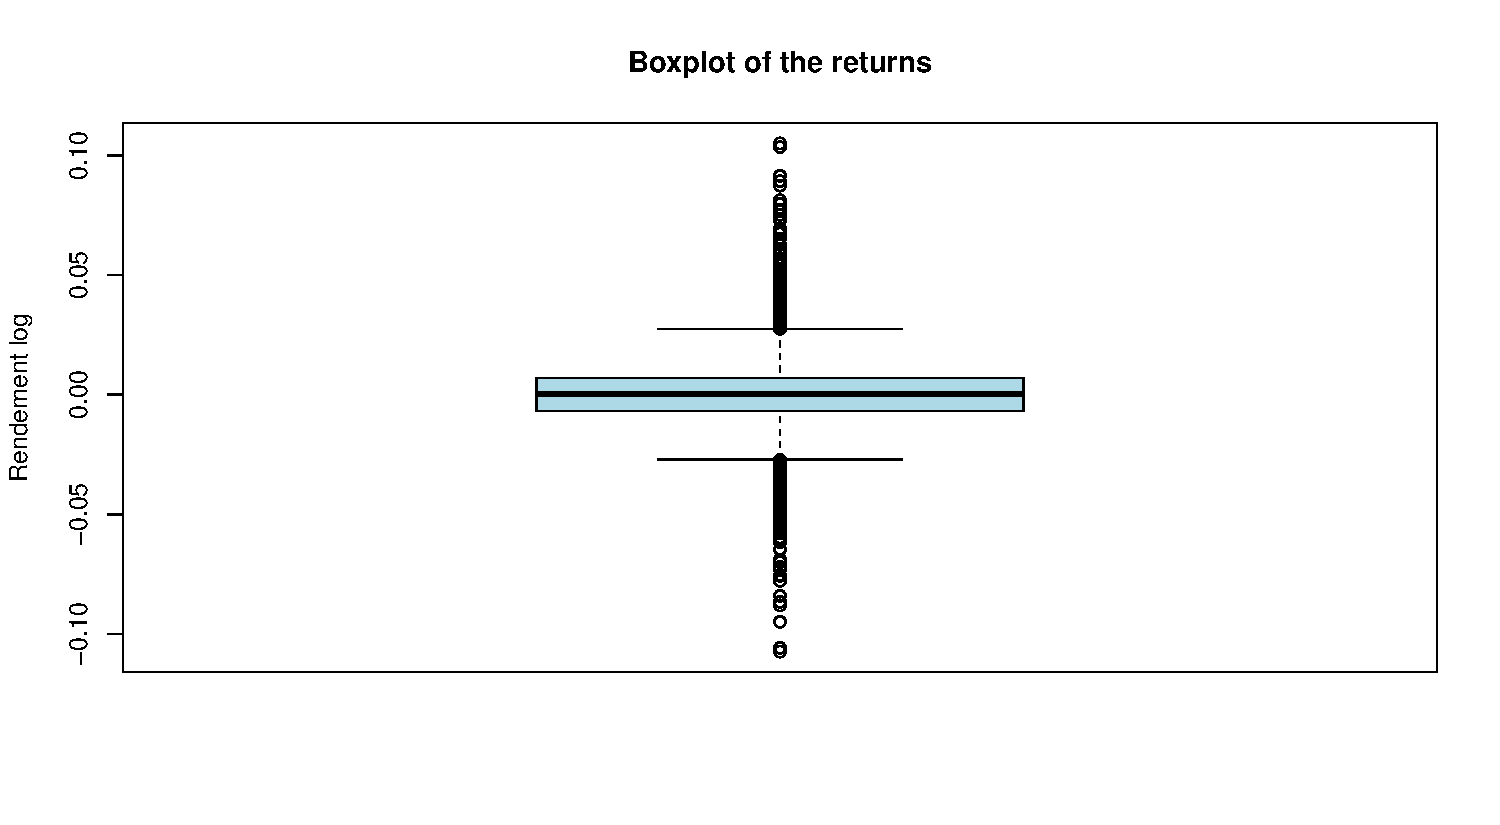
\includegraphics{QRM_files/figure-latex/unnamed-chunk-4-1.pdf}

The boxplot shows several outliers, which implies that the distribution
has heavy tails. The result of the Jarque-Bera test leads us to reject
the hypothesis of normality. These results highlight characteristics of
non-normality, which motivates the use of conditional volatility models,
such as GARCH.

\begin{verbatim}
## 
##  Jarque Bera Test
## 
## data:  log_returns
## X-squared = 11216, df = 2, p-value < 2.2e-16
\end{verbatim}

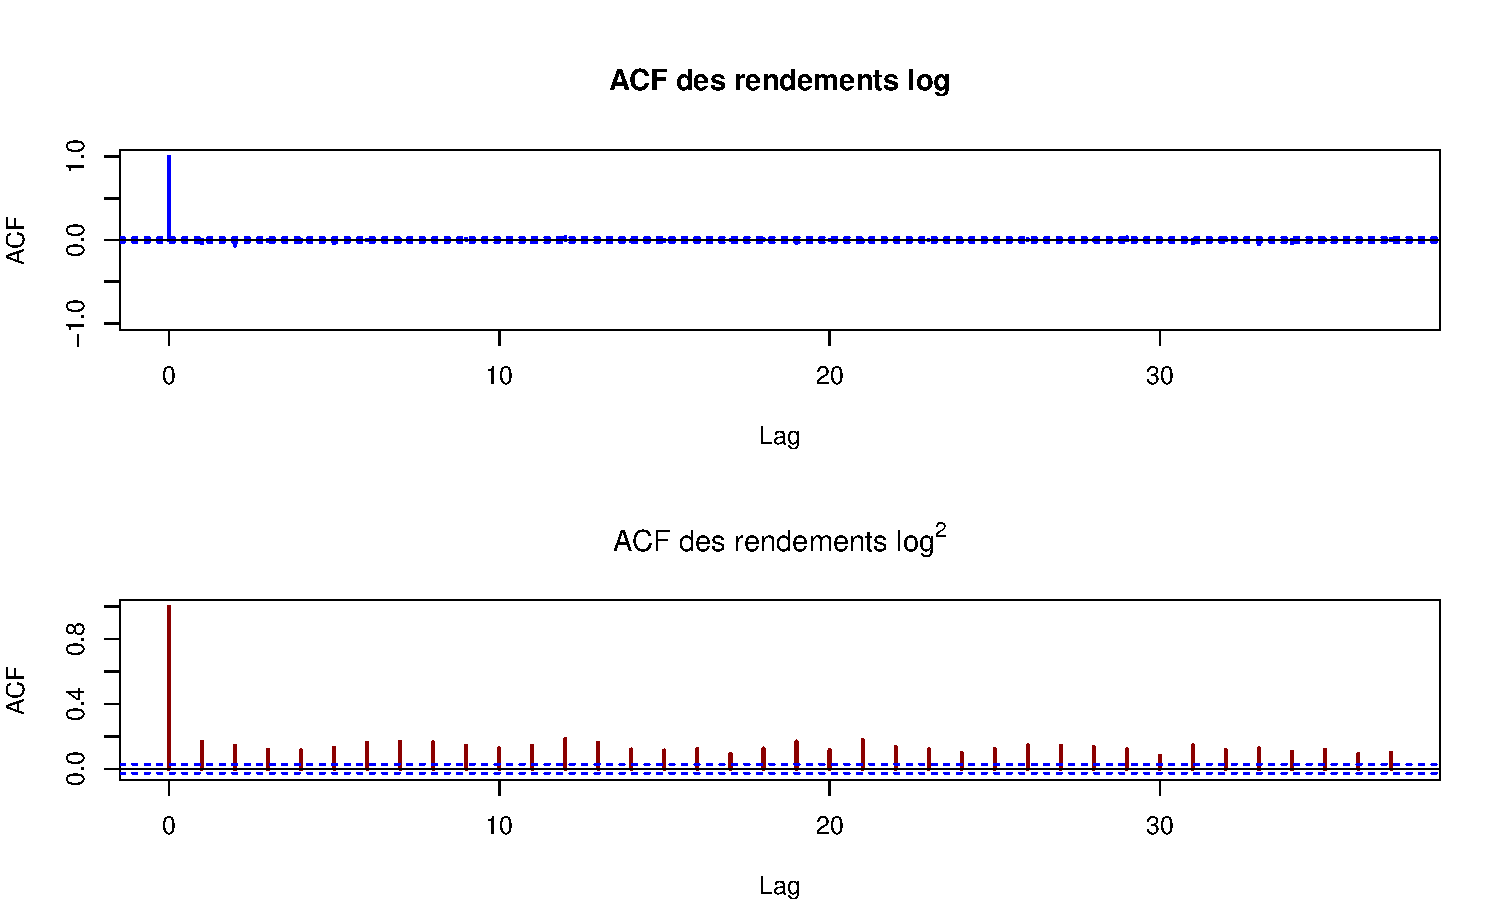
\includegraphics{QRM_files/figure-latex/unnamed-chunk-5-1.pdf}
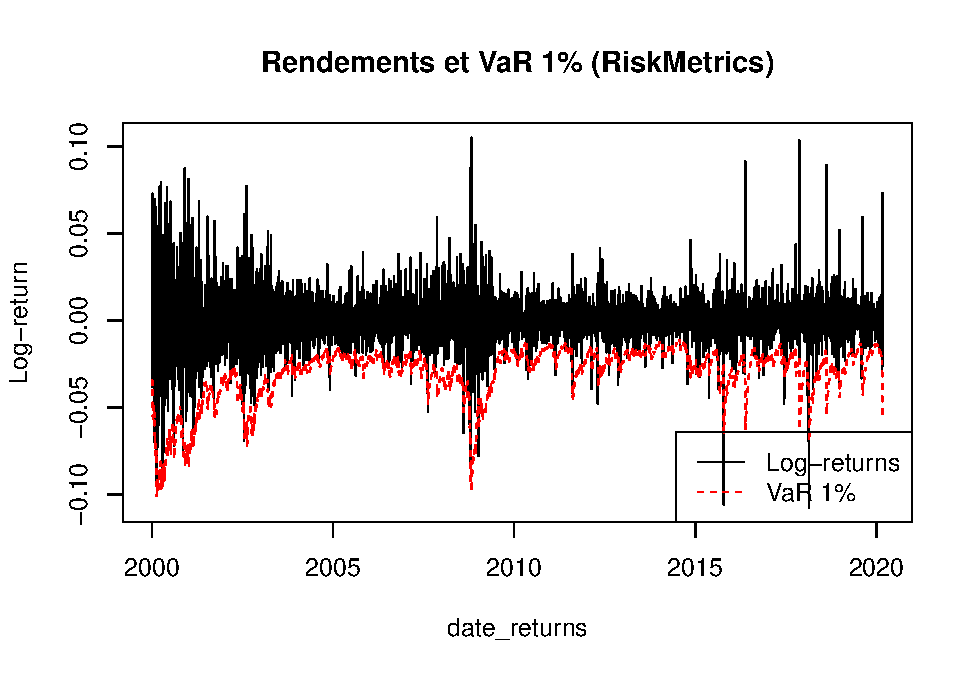
\includegraphics{QRM_files/figure-latex/unnamed-chunk-6-1.pdf}

\begin{verbatim}
## 
## Call:
## glm(formula = y_target ~ X - 1, family = binomial(link = "logit"))
## 
## Coefficients:
##    Estimate Std. Error z value Pr(>|z|)    
## X1  -3.5673     0.2495 -14.296  < 2e-16 ***
## X2  -0.4986     1.0134  -0.492  0.62273    
## X3   1.1279     0.4779   2.360  0.01827 *  
## X4   0.7106     0.5991   1.186  0.23560    
## X5   1.3541     0.4407   3.072  0.00212 ** 
## X6 -13.5207   401.7561  -0.034  0.97315    
## X7 -16.5145     8.2305  -2.006  0.04480 *  
## ---
## Signif. codes:  0 '***' 0.001 '**' 0.01 '*' 0.05 '.' 0.1 ' ' 1
## 
## (Dispersion parameter for binomial family taken to be 1)
## 
##     Null deviance: 7028.51  on 5070  degrees of freedom
## Residual deviance:  915.89  on 5063  degrees of freedom
## AIC: 929.89
## 
## Number of Fisher Scoring iterations: 16
\end{verbatim}

\begin{longtable}[]{@{}
  >{\raggedright\arraybackslash}p{(\columnwidth - 2\tabcolsep) * \real{0.4483}}
  >{\raggedright\arraybackslash}p{(\columnwidth - 2\tabcolsep) * \real{0.5517}}@{}}
\toprule\noalign{}
\begin{minipage}[b]{\linewidth}\raggedright
Coefficient
\end{minipage} & \begin{minipage}[b]{\linewidth}\raggedright
Interpretation
\end{minipage} \\
\midrule\noalign{}
\endhead
\bottomrule\noalign{}
\endlastfoot
X1 (Constant) & Highly significant (p \textless{} 2e-16) → indicates a
non-zero average probability of exception. \\
X2 to X6 (Lags of past exceptions) & Some are not significant (e.g.~X2,
X4, X6), but others are (X3, X5, X7). \\
X7 (VaR) & Significant at the 5\% level (p = 0.04480) → the probability
of exception depends on the VaR itself, which is not desirable. \\
\end{longtable}

\end{document}
